\chapter{METHODOLOGY}
\label{chap:methodology}

\section{System architecture overview}

The proposed Amazon Marketplace Intelligence framework is implemented
as a scheduled, modular data system. Its purpose is to collect Amazon
marketplace observations, store them in a relational warehouse, compute
interpretable analytical signals, and deliver those signals through both
dashboards and Telegram-based specialist agents. The implementation is
intentionally lightweight: it is designed as an operational thesis
prototype rather than a real-time streaming platform.

\subsection{High-level data flow}

The operational pipeline is organised as a sequential set of scheduled
data transformations. The architecture consists of four main tiers:
\begin{enumerate}
    \item \textbf{Data acquisition layer:} Apify actors collect Amazon
    category-ranking pages, product-detail snapshots, images, and recent
    review pages. The actors return JSON payloads, which are then parsed
    and validated by project-specific Python code.

    \item \textbf{Storage layer:} Raw and derived records are persisted
    in a Supabase PostgreSQL warehouse. Product images are stored in the
    Supabase Storage bucket \texttt{product-images}. All database access
    in the project code goes through the shared Supabase client defined
    in \texttt{lib/db.py}.

    \item \textbf{Analytical processing layer:} Python scripts under
    \texttt{scripts/} compute entrant/exit events, content and image
    changes, sponsored share-of-voice, K-Means price tiers, RoBERTa
    sentiment, Brand Momentum Score (BMS), Listing Quality Score (LQS),
    rule-based alerts, and Prophet price forecasts. The orchestration
    script \texttt{scripts/run\_analytics.py} executes these modules in
    a fixed dependency-aware order.

    \item \textbf{Multi-channel delivery layer:} A Streamlit dashboard
    supports internal analysis, a lightweight static web dashboard
    provides compact market overviews, and OpenClaw specialist agents
    deliver concise Telegram briefs. The agents do not write to the
    database; they call read-only Python skills that query Supabase and
    return JSON.
\end{enumerate}

The implementation relies on standard scientific Python libraries throughout all layers: NumPy \citep{harris2020numpy} and pandas \citep{mckinney2010pandas} for array and dataframe operations, Matplotlib \citep{hunter2007matplotlib} for figure generation, PyTorch \citep{paszke2019pytorch} as the backend for the Hugging Face \texttt{transformers} pipeline, and the \texttt{requests} \citep{requests2026docs}, \texttt{python-dotenv} \citep{pythondotenv2026}, and \texttt{PyYAML} \citep{pyyaml2025pypi} packages for HTTP communication, environment management, and configuration parsing respectively.

\begin{figure}[htbp]
  \centering
  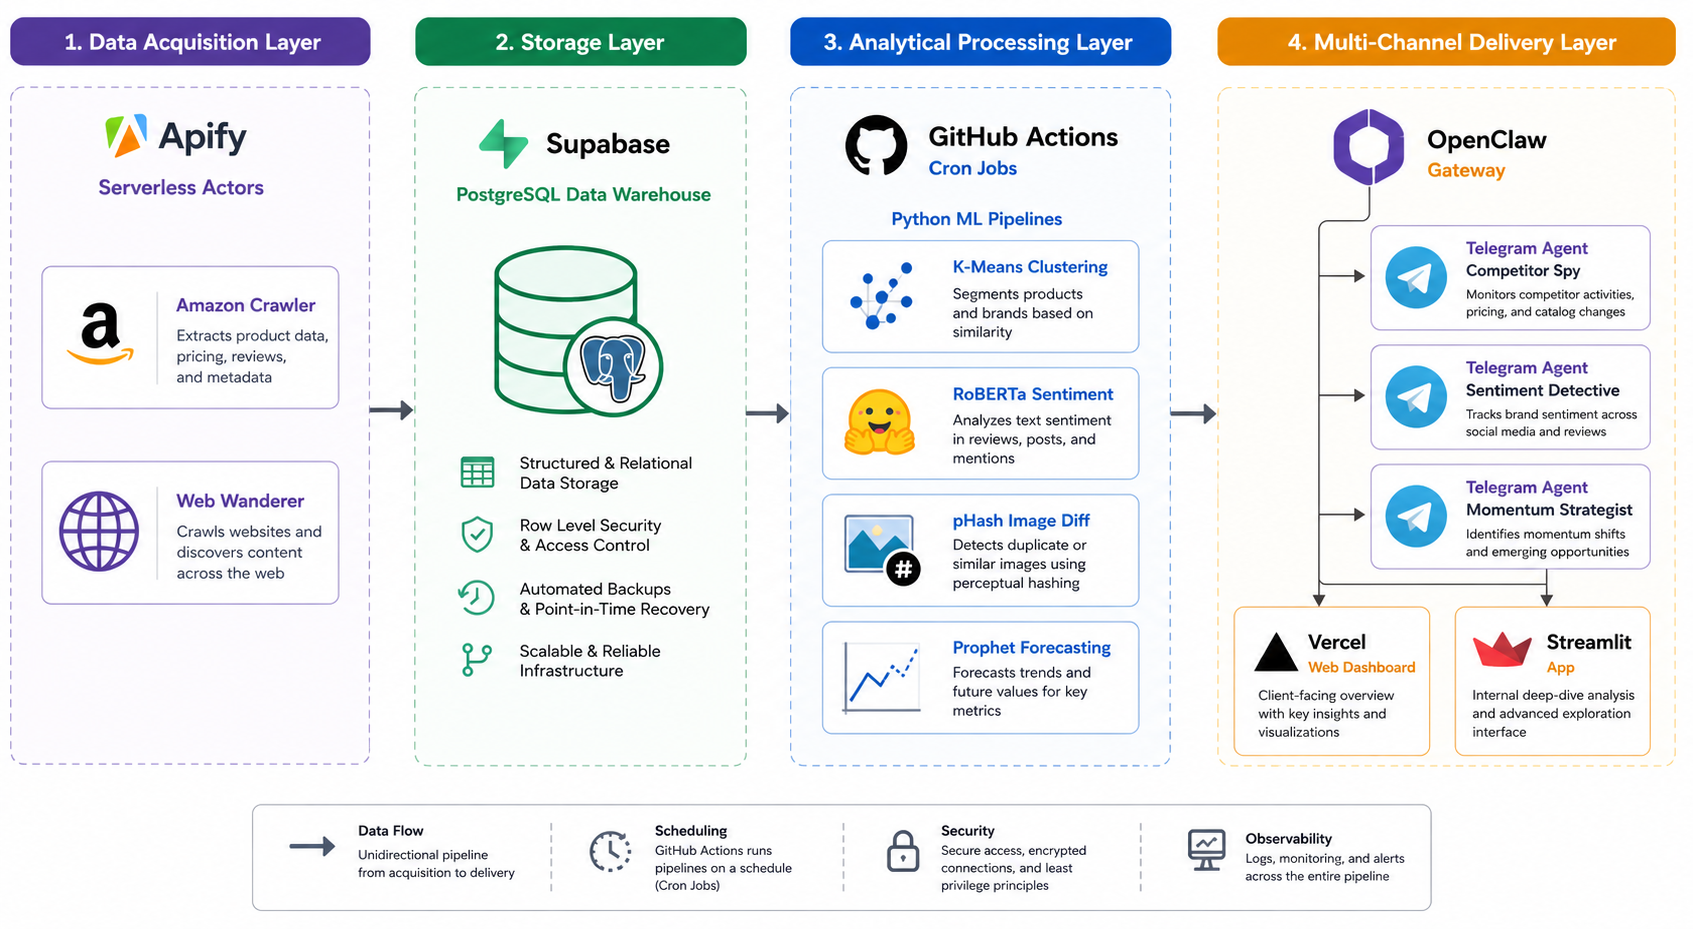
\includegraphics[width=\textwidth]{figures/architecture.png}
  \caption{System architecture overview, detailing the flow from data acquisition to the multi-channel delivery ecosystem.}
  \label{fig:architecture}
\end{figure}

\subsection{Database schema and storage mechanism}

The PostgreSQL database is managed through version-controlled SQL
migrations from \texttt{migrations/001\_new\_tables.sql} to\linebreak
\texttt{migrations/005\_price\_forecast.sql}. The helper function
\texttt{upsert()} in \texttt{lib/db.py} wraps Supabase table-level
upserts and returns the number of processed rows. This wrapper
centralises database access, but it is not a full ORM and does not
provide multi-statement database transactions. Consequently, steps that
require multiple operations, such as clearing and reinserting daily
alerts, are treated as pragmatic thesis-pipeline operations rather than
fully transactional production routines.

The analytical backbone depends on several tables. Two important tables
are \texttt{daily\_snapshots}, which stores product-level time-series
observations for the 30 watchlist ASINs, and \texttt{reviews\_raw}, which
stores parsed Amazon review records. Tables~\ref{tab:schema_daily_snapshots}
and~\ref{tab:schema_reviews_raw} show selected columns used by the
pipeline rather than every column in the database.

\begin{table}[H]
  \centering
  \small
  \begin{tabular}{p{3.2cm}l@{\hspace{6pt}}l@{\hspace{6pt}}p{5.8cm}}
    \toprule
    \textbf{Column Name} & \textbf{Data Type} & \textbf{Role} & \textbf{Description} \\
    \midrule
    \texttt{snapshot\_date} & \texttt{DATE} & Key & Ingestion date. \\
    \texttt{asin} & \texttt{TEXT} & Key & Amazon Standard Identification Number. \\
    \texttt{bsr} & \texttt{INT} & Signal & Best Sellers Rank parsed from product-detail data. \\
    \texttt{price} & \texttt{NUMERIC} & Signal & Current observed product price. \\
    \texttt{list\_price} & \texttt{NUMERIC} & Signal & Reference list price when present. \\
    \texttt{discount\_pct} & \texttt{NUMERIC} & Derived & Percentage discount when \texttt{list\_price > price}. \\
    \texttt{buy\_box\_winner} & \texttt{TEXT} & Signal & Seller name parsed from the actor output. \\
    \texttt{in\_stock} & \texttt{BOOLEAN} & Signal & Inventory availability; \texttt{NULL} means unknown. \\
    \texttt{has\_promo} & \texttt{BOOLEAN} & Signal & Promotional badge or sale summary detected. \\
    \texttt{stars} & \texttt{NUMERIC} & Signal & Average product rating. \\
    \texttt{reviews\_count} & \texttt{INT} & Signal & Total review count observed on the product page. \\
    \texttt{bullet\_count} & \texttt{INT} & Signal & Number of bullet features parsed from the listing. \\
    \texttt{image\_url} & \texttt{TEXT} & Signal & Supabase Storage URL or original image URL. \\
    \texttt{image\_hash} & \texttt{TEXT} & Derived & Perceptual hash of the main image. \\
    \texttt{image\_changed} & \texttt{BOOLEAN} & Derived & Daily image-change flag computed during watchlist ingest. \\
    \texttt{ebc\_html\_hash} & \texttt{TEXT} & Derived & MD5 hash of A+ content text when available. \\
    \texttt{stars\_breakdown} & \texttt{JSONB} & Signal & Percentage distribution of 1--5 star ratings. \\
    \bottomrule
  \end{tabular}
  \caption{Selected fields from \texttt{daily\_snapshots}.}
  \label{tab:schema_daily_snapshots}
\end{table}

\begin{table}[H]
  \centering
  \small
  \begin{tabular}{p{3.2cm}l@{\hspace{6pt}}l@{\hspace{6pt}}p{5.8cm}}
    \toprule
    \textbf{Column Name} & \textbf{Data Type} & \textbf{Role} & \textbf{Description} \\
    \midrule
    \texttt{id} & \texttt{BIGSERIAL} & PK & Internal review-row identifier. \\
    \texttt{asin} & \texttt{TEXT} & UK & Product ASIN receiving the review. \\
    \texttt{review\_id} & \texttt{TEXT} & UK & Amazon review identifier. \\
    \texttt{review\_date} & \texttt{DATE} & Signal & Review date parsed from the actor output. \\
    \texttt{rating} & \texttt{INT} & Signal & User-submitted star rating. \\
    \texttt{title} & \texttt{TEXT} & Signal & Review title. \\
    \texttt{review\_text} & \texttt{TEXT} & Signal & Review body used by RoBERTa. \\
    \texttt{verified} & \texttt{BOOLEAN} & Signal & Verified-purchase flag. \\
    \texttt{helpful\_votes} & \texttt{INT} & Signal & Helpful-vote count. \\
    \texttt{is\_vine} & \texttt{BOOLEAN} & Signal & Amazon Vine review flag. \\
    \texttt{has\_images} & \texttt{BOOLEAN} & Signal & Whether the review includes images. \\
    \texttt{country} & \texttt{TEXT} & Signal & Review country when present. \\
    \texttt{aspects\_json} & \texttt{JSONB} & Signal & Amazon product-level aspect summary when available. \\
    \texttt{sentiment\_label} & \texttt{TEXT} & Derived & RoBERTa label: positive, neutral, or negative. \\
    \texttt{sentiment\_score} & \texttt{NUMERIC} & Derived & Confidence-weighted sentiment scalar in $[-1,1]$. \\
    \bottomrule
  \end{tabular}
  \caption{Selected fields from \texttt{reviews\_raw}.}
  \label{tab:schema_reviews_raw}
\end{table}

\section{Data acquisition pipeline}

Amazon data extraction is delegated to Apify actors rather than a
custom Selenium or BeautifulSoup scraper. This choice reduces the
maintenance burden of dealing with dynamic Amazon pages and anti-bot
controls, while still requiring project-specific parsing, validation,
caching, and deduplication in Python. The actor outputs are treated as
structured inputs to the local pipeline, not as perfectly deterministic
or error-free records.

\subsection{Watchlist ingestion}

The watchlist pipeline is implemented in
\texttt{scripts/ingest\_watchlist.py}. It collects product-detail
snapshots for the 30 ASINs defined in \texttt{config.WATCHLIST}. The
ASINs are processed in batches of 10 through the
\texttt{junglee/Amazon-crawler} actor with
\texttt{scrapeProductDetails=True}, \texttt{maxItemsPerStartUrl=1}, and
\texttt{proxyCountry="AUTO\_SELECT\_PROXY\_COUNTRY"}.

To reduce unnecessary Apify cost during retry scenarios, the script
caches the raw actor output under \texttt{data/raw/watchlist\_<date>.json}.
If a later database write fails, the same raw data can be reused without
re-scraping the product pages. Each raw item is parsed by
\texttt{lib/parsers/product.py}, which extracts price, list price,
discount percentage, BSR, stock availability, seller, review count,
rating, bullet count, A+ content hash, and the main image URL. The
script also filters out records whose returned ASIN is not in the
watchlist, because search-based actor outputs can occasionally return a
different ASIN from the requested one.

\subsection{Category rankings ingestion}

The broader market-ranking pipeline is implemented in
\texttt{scripts/ingest\_category.py}. It runs the same Amazon crawler
actor over the three configured category search URLs:
\texttt{gaming\_keyboard}, \texttt{true\_wireless\_earbuds}, and
\texttt{portable\_charger}. For each category, the script requests the
Top 50 search-result records and writes the parsed rankings to
\texttt{category\_rankings}. Product metadata is also upserted into the
\texttt{asins} table.

The implementation deduplicates ranking rows by
(\texttt{snapshot\_date}, \texttt{browse\_node}, \texttt{rank}) because
the actor may occasionally return repeated positions. It also deduplicates
ASIN metadata before writing to \texttt{asins}. These daily category
snapshots support entrant/exit detection, price-tier clustering, and
sponsored share-of-voice estimation.

\subsection{Consumer reviews ingestion}

The review pipeline is implemented in
\texttt{scripts/ingest\_reviews.py}. It uses the
\texttt{web\_wanderer/amazon-reviews-extractor} actor to collect recent
English verified-purchase reviews for the 30 watchlist ASINs. The code
sets \texttt{pagesPerProduct = 2}, \texttt{sortBy = "recent"},
\texttt{languageFilter = "en"}, \texttt{verifiedPurchases = True}, and
\texttt{includeVariants = False}. The pipeline is therefore a recent-page
refresh with upsert-based deduplication by \texttt{(asin, review\_id)},
not a cursor-based incremental crawler.

Parsed reviews are stored in \texttt{reviews\_raw}. When the actor
returns Amazon aspect summaries, they are stored in
\texttt{aspects\_json}. The script also extracts product-level review
summaries into \texttt{product\_review\_summary} when that table is
available. This distinction matters: the project does not train a custom
aspect-based sentiment model; it uses Amazon-provided aspect summaries
as an additional marketplace signal.

\subsection{Target categories and watchlist}

Three consumer-electronics sub-categories were selected because they
show frequent ranking changes, meaningful price variation, and sufficient
review availability. The final watchlist contains 10 ASINs per category,
for 30 watchlist products in total. It covers established and emerging
brands observed in the selected categories, including Logitech,
Redragon, AULA, Soundcore, TOZO, JBL, Apple, Samsung, Anker, INIU,
Charmast, VEGER, and related direct-to-consumer brands.

\begin{table}[H]
  \centering
  \begin{tabular}{llc}
    \toprule
    \textbf{Category} & \textbf{Search URL} & \textbf{Scope} \\
    \midrule
    Gaming Keyboards      & amazon.com/s?k=gaming+keyboard       & Top 50 + 10 watchlist \\
    True Wireless Earbuds & amazon.com/s?k=true+wireless+earbuds & Top 50 + 10 watchlist \\
    Portable Chargers     & amazon.com/s?k=portable+charger      & Top 50 + 10 watchlist \\
    \bottomrule
  \end{tabular}
  \caption{Target categories and collection scope.}
  \label{tab:categories}
\end{table}

\subsection{Image processing pipeline}

Image handling occurs during watchlist ingestion and later during the
analytics pass. During ingestion, the parser selects the first
high-resolution image when available, falling back to the thumbnail. The
image is downloaded, converted to RGB through Pillow, hashed using
\texttt{imagehash.phash()}, and uploaded to the Supabase Storage bucket
\texttt{product-images} at the path
\texttt{YYYY-MM-DD/ASIN/main.jpg}. The current pHash is compared with
yesterday's stored pHash; if the Hamming distance exceeds
\texttt{config.PHASH\_THRESHOLD = 10}, the daily snapshot receives
\texttt{image\_changed=True}.

The later script \texttt{scripts/analyze\_changes.py} independently
compares today's and yesterday's hashes and persists significant changes
to \texttt{image\_change\_events}. It also detects content changes in
A+ content hashes and bullet counts, writing those events to
\texttt{content\_change\_events}.

\subsection{Data quality and validation}

The implemented pipeline applies several pragmatic data-quality checks:
\begin{itemize}
    \item \textbf{Environment validation:} ingestion scripts call
    \texttt{require\_env()} to fail fast when required secrets such as
    \texttt{APIFY\_TOKEN}, \texttt{SUPABASE\_URL}, or
    \texttt{SUPABASE\_KEY} are missing.
    \item \textbf{Parser normalisation:} product and category parsers
    normalise prices, BSR values, stock fields, review counts, and image
    URLs into consistent row dictionaries.
    \item \textbf{Wrong-ASIN filtering:} watchlist records are filtered
    against the configured ASIN set before writing to
    \texttt{daily\_snapshots}.
    \item \textbf{Deduplication:} category rankings are deduplicated by
    date, category, and rank; reviews are upserted by ASIN and review ID.
    \item \textbf{Review batch diagnostics:} the review parser logs
    missing text, missing ASINs, missing review IDs, non-English records,
    and aspect availability before upsert.
    \item \textbf{Database constraints:} SQL migrations define uniqueness
    constraints and selected \texttt{CHECK} constraints for event type,
    severity, and change category.
\end{itemize}

The code uses console logging through \texttt{print()} statements rather
than a structured logging framework, and it does not include a formal
unit-test suite. These are acceptable limitations for the thesis
prototype but should be improved in a production version.

\subsection{Pipeline schedules and cost profile}

The data and analytics jobs are implemented in one GitHub Actions
workflow, \texttt{.github/workflows/daily\_ingest.yml}, with multiple
scheduled and manual-dispatch jobs. The daily job runs at 06:00 UTC
(13:00 ICT) and performs category ingestion, watchlist ingestion, and the
full analytics chain. A separate Monday schedule at 07:00 UTC runs the
review collection and sentiment-analysis job. Manual dispatch supports
\texttt{full}, \texttt{analytics\_only}, and \texttt{forecast\_only}
modes, allowing analytics and Prophet debugging without re-consuming
Apify credits.

\begin{table}[htbp]
  \centering
  \small
  \resizebox{\textwidth}{!}{%
  \begin{tabular}{llll}
    \toprule
    \textbf{Job} & \textbf{Schedule} & \textbf{Owner} & \textbf{Purpose} \\
    \midrule
    \texttt{ingest} & 06:00 UTC daily & GitHub Actions & Category rankings, watchlist snapshots, analytics chain. \\
    \texttt{reviews} & 07:00 UTC Monday & GitHub Actions & Recent reviews and RoBERTa sentiment analysis. \\
    \texttt{analytics\_only} & Manual dispatch & GitHub Actions & Re-run analytics without Apify scraping. \\
    \texttt{forecast\_only} & Manual dispatch & GitHub Actions & Re-run Prophet forecast and Supabase upsert. \\
    \texttt{daily-brief-strategist} & 08:00 ICT daily & OpenClaw & Strategist Telegram brief. \\
    \texttt{weekly-competitor-spy} & 09:00 ICT Monday & OpenClaw & Competitor recap. \\
    \texttt{weekly-sentiment-detective} & 09:00 ICT Wednesday & OpenClaw & Sentiment digest. \\
    \bottomrule
  \end{tabular}}%
  \caption{Pipeline schedule across GitHub Actions and OpenClaw cron jobs.}
  \label{tab:schedules}
\end{table}

Operating the pipeline at the configuration used in this thesis incurs
low monthly cost because Supabase, GitHub Actions, Telegram, and the
self-hosted OpenClaw runtime are used within free or near-free tiers.
The main recurring cost is Apify usage, with a small additional cost for
\texttt{gpt-5.4-mini} calls through the OpenClaw Gateway.

\begin{table}[H]
  \centering
  \small
  \begin{tabular}{lll}
    \toprule
    \textbf{Service} & \textbf{Tier} & \textbf{Monthly cost} \\
    \midrule
    Apify Amazon actors & Pay-as-you-go & $\sim$ \$8--10 \\
    Supabase PostgreSQL & Free tier & \$0 \\
    Supabase Storage & Free tier & \$0 \\
    GitHub Actions & Free tier & \$0 \\
    OpenClaw runtime & Self-hosted VMware & \$0 \\
    Telegram Bot API & Free & \$0 \\
    OpenAI \texttt{gpt-5.4-mini} & Pay-as-you-go & $<$ \$1 \\
    \midrule
    \textbf{Total} & & \textbf{$<$ \$11} \\
    \bottomrule
  \end{tabular}
  \caption{Monthly operating cost profile.}
  \label{tab:costs}
\end{table}

\section{Analytical components and machine learning pipelines}

The analytics chain is executed by \texttt{scripts/run\_analytics.py} in
the following order: entrant/exit detection, content and image changes,
sponsored share, price-tier clustering, sentiment aggregation, BMS, LQS,
alerts, and price forecasting. This ordering is necessary because BMS
and LQS depend on sentiment aggregates, while the alert layer depends on
daily snapshots and entrant/exit events.

\subsection{Image difference detection (pHash)}

The framework uses perceptual hashing to detect meaningful changes in
main product images. The implementation calls
\texttt{imagehash.phash()} and compares two 64-bit hash strings using
Hamming distance:
\begin{equation}
    d_H(h_t, h_{t-1}) =
    \sum_{i=1}^{64} \mathbb{1}\left(h_t^{(i)} \neq h_{t-1}^{(i)}\right).
\end{equation}
The configured threshold is $d_H > 10$. During ingestion, this threshold
sets the daily \texttt{image\_changed} flag. During the analytics pass,
\texttt{scripts/analyze\_changes.py} writes qualifying changes to
\texttt{image\_change\_events}. pHash is suitable for detecting that a
visual redesign occurred, but it does not explain the semantic content
of the redesign.

\subsection{Sentiment analysis (RoBERTa)}

The sentiment pipeline uses
\texttt{\seqsplit{cardiffnlp/twitter-roberta-base-sentiment-latest}} through the
Hugging Face \texttt{transformers} pipeline. For each unlabelled review,
the model returns a class label and confidence score. The implementation
stores both a discrete label and a signed scalar:
\begin{equation}
    s =
    \text{confidence} \times
    \begin{cases}
      +1 & \text{if label = positive},\\
      0  & \text{if label = neutral},\\
      -1 & \text{if label = negative}.
    \end{cases}
\end{equation}
This scalar \texttt{sentiment\_score} lies in $[-1,1]$ and is used by
both BMS and LQS.

Daily sentiment aggregation is performed by
\texttt{aggregate\_to\_daily()} in \texttt{scripts/analyze\_sentiment.py}.
The implementation aggregates all reviews that have been analysed for
each ASIN, not only reviews newly collected on that specific day.
Therefore, the database field \texttt{review\_count\_new} should be
interpreted as the current analysed review count in the aggregate, not a
strict count of newly added reviews.

\subsection{Price tier clustering (K-Means)}

The price-tier module applies univariate K-Means clustering to product
prices within each category's current Top-50 records. Prices are
standardised with \texttt{StandardScaler}, clustered with scikit-learn
\texttt{KMeans(n\_clusters=k, random\_state=42, n\_init=10)}, and then
mapped to entry, mid, and premium tiers by sorting the inverse-transformed
cluster centres.

The intended value is $k=3$, but the code uses
$k=\min(3,\text{number of unique prices})$. If fewer than two unique
prices are available, all products in that category snapshot are assigned
to the entry tier. This fallback prevents the pipeline from failing on
thin or degenerate price data.

\subsection{Time-series price forecasting (Prophet)}

The price-forecasting module uses Prophet with the \texttt{CMDSTANPY}
backend. Production forecasting and evaluation use different minimum
history requirements. In \texttt{scripts/analyze\_price\_forecast.py},
an ASIN is forecast if it has at least three historical price points. The
model disables daily, weekly, and yearly seasonality:
\begin{equation}
    y(t) = g(t) + \epsilon_t,
\end{equation}
where $g(t)$ is the fitted trend and $\epsilon_t$ is the residual error.
The model then produces a 7-day forecast with \texttt{yhat},
\texttt{yhat\_lower}, and \texttt{yhat\_upper}. Forecasts are written both
to \texttt{data/forecasts/} and, more importantly, to the
\texttt{price\_forecast\_daily} Supabase table. The Supabase table is the
canonical source for OpenClaw, because GitHub Actions and the OpenClaw VM
run on different machines.

Evaluation is stricter. \texttt{scripts/evaluate\_forecast.py} requires
at least \texttt{MIN\_HISTORY + HOLDOUT = 10} price observations, holds
out the final three days, trains on the earlier observations, and reports
MAE, MAPE, naive last-value MAE, and 80\% prediction-interval coverage.
This is a temporal holdout backtest rather than a repeated rolling
backtest.

\subsection{Brand Momentum Score (BMS)}

The Brand Momentum Score is computed in \texttt{scripts/analyze\_bms.py}.
It combines BSR velocity, review-count velocity, and sentiment into a
daily momentum indicator. The raw BSR velocity is
\begin{equation}
    v_{\text{BSR}} = \frac{\text{BSR}_{t-1} - \text{BSR}_{t}}
    {\text{BSR}_{t-1}},
\end{equation}
so an improvement in rank produces a positive value. The implementation
normalises the three inputs as follows:
\begin{align}
    n_{\text{BSR}} &= \text{clip}\left(\frac{v_{\text{BSR}} + 1}{2},0,1\right),\\
    n_{\text{review}} &= \text{clip}\left(\frac{\text{reviews}_{t} - \text{reviews}_{t-1}}{50},0,1\right),\\
    n_{\text{sent}} &= \frac{\text{sentiment}+1}{2}.
\end{align}
If BSR or sentiment is unavailable, the code defaults the corresponding
normalised signal to 0.5. The final score is
\begin{equation}
    \text{BMS} =
    0.5 n_{\text{BSR}} +
    0.3 n_{\text{review}} +
    0.2 n_{\text{sent}}.
\end{equation}
BMS should be interpreted as a transparent daily ranking heuristic, not
as a causal sales model.

\subsection{Listing Quality Score (LQS)}

The Listing Quality Score is computed in \texttt{scripts/analyze\_lqs.py}
as an additive 0--100 point score. Seven components are active in the
current implementation:
\begin{itemize}
    \item title score: up to 10 points, full score at 10 or more words;
    \item bullet score: up to 15 points, full score at 5 or more bullets;
    \item image score: 15 points if an image URL is present;
    \item A+ content score: 15 points if \texttt{ebc\_html\_hash} exists;
    \item rating score: up to 20 points, computed as \texttt{stars}/5;
    \item review score: up to 15 points, capped at 1,000 reviews;
    \item sentiment score: up to 10 points, based on the normalised sentiment scalar.
\end{itemize}
The database schema also contains \texttt{video\_score} and
\texttt{freshness\_score}, but the current code sets both to zero. They
are reserved fields rather than active score components in this thesis.

LQS should be interpreted as a transparent descriptive heuristic rather than a validated quality metric. The component weights (10, 15, 15, 15, 20, 15, 10) were chosen to reflect conventional Amazon seller guidance and sum to 100 for interpretability; they have not been estimated from sales or ranking data. The score is most useful for identifying listing outliers and tracking changes over time within a fixed watchlist, not for cross-category comparison or causal claims about ranking outcomes.

\subsection{Rule-based alerts}

The alert engine in \texttt{scripts/analyze\_alerts.py} converts selected
market events into operational alerts. The implemented rules are:
\begin{itemize}
    \item \texttt{price\_drop}: price falls by at least 15\% in one day;
    severity is high if the drop is at least 30\%, otherwise medium;
    \item \texttt{stockout}: \texttt{in\_stock} changes from true
    yesterday to false today; severity is high;
    \item \texttt{bsr\_drop}: BSR worsens by more than 500 positions;
    severity is medium;
    \item \texttt{image\_change}: daily snapshot indicates image change;
    severity is low;
    \item \texttt{new\_entrant}: ASIN enters the Top 50; severity is high
    for Top-10 entrants and low otherwise;
    \item \texttt{exit}: ASIN exits the Top 50; severity is medium.
\end{itemize}
Before inserting alerts, the script deletes existing alerts for the same
snapshot date to avoid duplicates on reruns. This is pragmatic
idempotency for the current thesis pipeline, not a fully transactional
production alerting design.

\section{Multi-agent delivery system (OpenClaw)}

The OpenClaw layer converts analytical outputs into short Telegram
briefs. It is best understood as a tool-using delivery layer over
Supabase, not as an autonomous system that directly mutates data.

\subsection{Agentic framework and gateway}

The OpenClaw Gateway connects Telegram accounts, LLM prompts, and
registered tools. The deployment uses one-to-one channel binding: each
Telegram bot account is bound to one specialist agent. This avoids the
need for keyword routing inside a single bot and keeps each agent's
persona, allowed skills, and output contract isolated.

\subsection{Specialist agents}

The three deployed agents are:
\begin{enumerate}
    \item \textbf{Competitor Spy (\texttt{@babyspyyy\_bot}):} Uses six
    skills: \texttt{query\_bms}, \texttt{query\_rankings},
    \texttt{query\_entrant\_exits}, \texttt{query\_sponsored\_share},
    \texttt{query\_price\_tiers}, and \texttt{query\_image\_changes}.

    \item \textbf{Sentiment Detective (\texttt{@babydetective\_bot}):}
    Uses four skills: \texttt{query\_sentiment}, \texttt{query\_reviews},
    \texttt{query\_aspects}, and \texttt{query\_snapshots}.

    \item \textbf{Momentum Strategist (\texttt{@babystrategist\_bot}):}
    Uses five skills: \texttt{query\_alerts}, \texttt{query\_bms},
    \texttt{query\_price\_forecast}, \texttt{query\_lqs}, and
    \texttt{query\_sentiment}.
\end{enumerate}

\subsection{Skill executions (tools)}

The project registers 13 read-only Python skills under
\texttt{openclaw/skills/}, with wrapper definitions under
\texttt{openclaw/wrappers/}. Each skill exposes a \texttt{SKILL}
metadata dictionary, a \texttt{run(**kwargs)} function, and a CLI
contract in which JSON arguments are passed to the script and JSON is
printed to \texttt{stdout}. Examples include \texttt{query\_bms},
\texttt{query\_price\_forecast}, and \texttt{query\_sentiment}.

The LLM does not receive direct write access to Supabase. Instead, within
each bound agent, the prompt and allowed-skill list constrain which
read-only skills may be called. This design reduces hallucination risk:
recommendations are expected to cite ASINs, dates, metrics, and values
returned by the skills rather than unsupported model memory.

\section{Evaluation methodology}
\label{sec:eval}

Two analytical modules produce predictions that require explicit
evaluation: the RoBERTa sentiment classifier and the Prophet price
forecaster.

\subsection{Sentiment classification: distant supervision against stars}

Because no manually labelled in-domain sentiment dataset is available,
the evaluation uses star ratings as noisy labels:
\begin{equation}
  y_{\text{star}} = \begin{cases}
    \text{negative} & \text{if rating} \in \{1, 2\}, \\
    \text{neutral}  & \text{if rating} = 3, \\
    \text{positive} & \text{if rating} \in \{4, 5\}.
  \end{cases}
\end{equation}
The evaluation script reports accuracy, per-class precision and recall,
per-class F\textsubscript{1}, macro-F\textsubscript{1}, and a
$3 \times 3$ confusion matrix. Macro-F\textsubscript{1} is important
because Amazon reviews are skewed toward positive ratings:
\begin{equation}
  \text{macro-F}_1 = \frac{1}{3}
  \sum_{c \in \{\text{negative}, \text{neutral}, \text{positive}\}}
    \frac{2 P_c R_c}{P_c + R_c}.
\end{equation}
The result should be interpreted as a noisy operational check, not a
perfect estimate of the model's true semantic understanding.

\subsection{Price forecasting: temporal holdout backtest}

For forecast evaluation, \texttt{scripts/evaluate\_forecast.py} uses a
temporal holdout protocol. For each eligible watchlist ASIN with at
least 10 price observations, the final $H=3$ days are held out, Prophet
is fitted on the earlier observations, and predictions are compared with
actual holdout prices. For each ASIN:
\begin{align}
  \text{MAE}_i  &= \frac{1}{H}\sum_t |y_{i,t} - \hat{y}_{i,t}|, \\
  \text{MAPE}_i &= \frac{1}{H}\sum_t
  \frac{|y_{i,t} - \hat{y}_{i,t}|}{y_{i,t}} \times 100\%.
\end{align}
The script also reports naive last-value MAE and 80\% prediction-interval
coverage. This makes it possible to disclose whether Prophet improves on
a simple carry-forward baseline under the short observation window.

\section{Hyperparameter and threshold selection}
\label{sec:hparams}

Table~\ref{tab:hparams} summarises the main hyperparameters and
thresholds implemented in the codebase.

\begin{table}[htbp]
  \centering
  \small
  \resizebox{\textwidth}{!}{%
  \begin{tabular}{p{3.4cm}p{2.6cm}p{7.0cm}}
    \toprule
    \textbf{Module} & \textbf{Setting} & \textbf{Implementation rationale} \\
    \midrule
    Category scrape & Top 50 & Matches the monitored ranking scope in \texttt{config.CATEGORIES}. \\
    Watchlist scrape & 30 ASINs, batch 10 & Three categories with 10 ASINs each; batch size controls Apify request size. \\
    Review scrape & 2 pages/product & Recent-page refresh to control Apify cost. \\
    K-Means tiering & $k \leq 3$, \texttt{n\_init=10} & Entry/mid/premium segmentation with thin-data fallback. \\
    pHash image diff & $d_H > 10$ & Configured in \texttt{config.PHASH\_THRESHOLD}. \\
    Sentiment model & Pretrained RoBERTa & No manually labelled in-domain training set available. \\
    Prophet forecast & $\geq 3$ price points & Minimum in \texttt{analyze\_price\_forecast.py}. \\
    Prophet eval & 3-day holdout, min 10 obs. & Implemented in \texttt{evaluate\_forecast.py}. \\
    BMS weights & $0.5, 0.3, 0.2$ & BSR velocity, review velocity, sentiment. \\
    LQS weights & $10,15,15,15,20,15,10$ & Title, bullets, image, A+, rating, reviews, sentiment. \\
    Alert: price drop & $\geq 15\%$; high $\geq 30\%$ & Implemented in \texttt{analyze\_alerts.py}. \\
    Alert: BSR drop & $>500$ positions & Implemented in \texttt{analyze\_alerts.py}. \\
    Alert: stockout & true-to-false transition & Implemented in \texttt{analyze\_alerts.py}. \\
    \bottomrule
  \end{tabular}}%
  \caption{Hyperparameters and decision thresholds across the analytical pipeline.}
  \label{tab:hparams}
\end{table}

These settings should be interpreted as transparent thesis heuristics.
They are fixed for reproducibility and interpretability rather than
estimated as globally optimal parameters.
